\documentclass[a4paper, 12pt, parskip]{scrreprt}

\def\Title{Code-Reuse Attacks for the Web: Breaking Cross-Site Scripting Mitigations via Script Gadgets}
\def\Author{Burhan Otour}
\def\Type{Seminar Thesis}
\def\Supervisor{Peter Chvojka} 

\usepackage[utf8]{inputenc}
\usepackage[english]{babel}
\usepackage{graphicx}
\usepackage{color}
\usepackage{xcolor}
\usepackage{listings}
\usepackage{todonotes}
\usepackage[
backend=bibtex,
style=numeric,
sorting=ynt
]{biblatex}
\addbibresource{bib/references.bib}
\newcommand\myworries[1]{\textcolor{red}{#1}}
% BEGIN: Code listing support for JavaScript 
\definecolor{lightgray}{rgb}{.9,.9,.9}
\definecolor{darkgray}{rgb}{.4,.4,.4}
\definecolor{purple}{rgb}{0.65, 0.12, 0.82}
\definecolor{c}{rgb}{1, 1, 1}

\lstdefinelanguage{JavaScript}{
	keywords={typeof, new, true, false, catch, function, return, null, catch, switch, var, if, in, while, do, else, case, break},
	keywordstyle=\color{blue}\bfseries,
	ndkeywords={class, export, boolean, throw, implements, import, this},
	ndkeywordstyle=\color{purple}\bfseries,
	identifierstyle=\color{black},
	sensitive=false,
	comment=[l]{//},
	morecomment=[s]{/*}{*/},
	commentstyle=\color{darkgray}\ttfamily,
	stringstyle=\color{red}\ttfamily,
	morestring=[b]',
	morestring=[b]"
} 

\lstset{
	language=JavaScript,
	backgroundcolor=\color{white},
	extendedchars=true,
	basicstyle=\footnotesize\ttfamily,
	showstringspaces=false,
	showspaces=false,
	numbers=left,
	numberstyle=\footnotesize,
	numbersep=9pt,
	tabsize=2,
	breaklines=true,
	showtabs=false,
	captionpos=b,
	frame=lines
}
% END: Code listing support for JavaScript

\begin{document}
	%%%
% LaTeX Template for Thesis submitted to AG-Jager
% This is just a guideline - modify as you like :)
% Last Update: 2‚4-05-2017
% Template provided by Kai Gellert
%%%

\begin{titlepage}
	\centering
	\begin{minipage}{14cm}		
		\hspace*{1.9cm}
		
\includegraphics[height=3cm]{figures/upb_logo}\\
		\hspace*{4cm}
		\begin{minipage}{9.5cm}
			\vspace*{5pt}
			\textsf{\noindent
				Fakultät für Elektrotechnik, Informatik und Mathematik\\
				Arbeitsgruppe IT-Sicherheit
			}
		\end{minipage}		
	\end{minipage}\\[50pt]
	{\Large\bfseries \Type\par}
	\vspace{1.5cm}
	{\huge\sffamily\bfseries{\Title}\par}
	\vspace{2cm}
	{\Large \Author\par}
	\vfill
	\begin{tabular}{r l}
		Date:    & \today \\
		Supervisor: & \Supervisor\\
	\end{tabular}
	\vfill
\end{titlepage}

	\pagenumbering{roman}
	
	\section*{Abstract}
		Over the past years, various Cross-site scripting (XSS) mitigation techniques were developed to tackle the problem of code injection vulnerabilities present in web application code bases.  The majority of these mitigations, however, share an assumption that says preventing XSS happens when detecting and blocking execution of illegitimate injected JavaScript code. This assumption slowly becomes a limitation to mitigations as modern JavaScript libraries and code patterns are introduced, which in turn expand the vulnerability vector in a way current XSS prevention techniques can’t recognize.\todo{Need to be fixed and expanded} 
	
	\clearpage
	
	\tableofcontents
	
	\clearpage
	
	\pagenumbering{arabic}

	\chapter{Introduction}
This is the introduction. %\include{content}
More detailed than the Abstract page. Here a general introduction to the topic is presented and a clear acknowledge of how the document is structured will be delivered.
\todo{Need to be added}
	
	\chapter{Background}
\todo{Add some text here}
\section{Cross-site scripting}
\textit{Cross-site scripting} (or \textit{XSS} for short) is a special type of code injection attack in the Web. In XSS, the attacker tries to inject arbitrary (and probably harmful) JavaScript code into web pages that will eventually be displayed on one victim browser\footnotemark . Once the targeted browser receives the web page, it will execute all its contained JavaScript code including the injected malicious payload which, of course, has exactly the same privileges as any other legitimate JavaScript code exists in that page.

\begin{figure}
	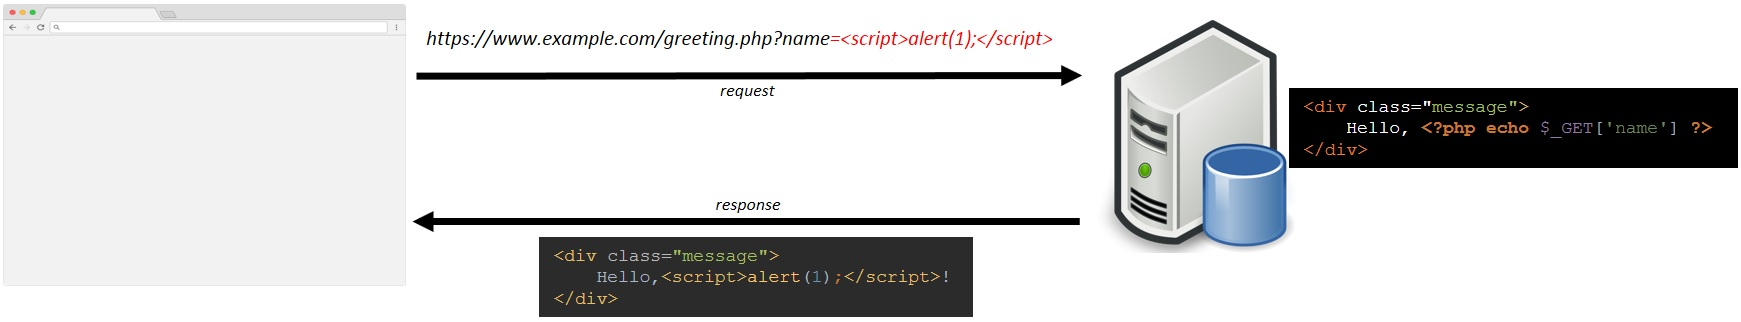
\includegraphics[width=\linewidth]{figures/xss_example.jpg}
	\caption{An example of reflected XSS attack}
	\label{fig:xss_example}
\end{figure}

Usually, XSS attack occurs as a result of exploiting a code injection vulnerability that persists in the target web application. In figure \ref{fig:xss_example}\todo{enlarge font in figure}, a PHP code snippet is responsible for displaying a small greeting message for the user. The value of the name is shipped within the name GET parameter and is included as part of the request URL. One attacker can induce the victim user to call an attacker-crafted request URL with the malicious payload being set to the name parameter. Without any string escaping mechanism or input filtering of the name value, the web application will simply inject that payload into the \verb!$_GET[‘name’]! placeholder once it receives the request and send the resultant HTML page back to the victim browser, which will in turn detect the injected script tag and executes its content resulting in XSS attack.

\footnotetext{Two types of XSS script injection mechanisms exist, namely Stored XSS and Reflected XSS. However, since injection techniques are out of the scope of this study, we omitted them from the discussion}

\section{XSS mitigations}
If we looked back at the vulnerable back-end code in figure \ref{fig:xss_example}, one can simply propose a code fix by which we filter out the input for any \verb|<script>| tag before it’s injected in the page. This filtering functionality will then be part of the web application logic. In real-world web applications, the web security community proposed a lot of secure code practices and standards to avoid such vulnerabilities (auto escaping templating systems, reporters and scanners)\footnotemark\todo{Need to add footnote text}. Nevertheless, at large scale, the process of detecting and fixing code injection bugs become a tedious task. Moreover, It was proven (cite) that it’s extremely difficult, at a large scale, to have a 100\% injection-bug-free web apps. Here is where XSS mitigations come into play. XSS mitigations share a very fundamental assumption; “XSS mitigations focus on preventing the attack instead of fixing the vulnerability”. So instead of looking for bugs, it tries to stop the attack itself, thus the application remains secure regardless of vulnerabilities existence. 

In our study, we consider four types of those mitigations:

\paragraph{Web application firewall WAFs} WAFs are placed in the server side, and provide filtering mechanism in which they look at all web traffic that come to the server and then apply a bunch of rules or regular expressions onto these requests in order to find potentially-malicious injected payloads. 
One well-known WAF that is heavily adopted in practice is ModSecurity  which is usually shipped with OWASP Core Rule Set (CRS); \todo{Need to be more specific here} a default set of detection and prevention rules for a wide range of XSS attack vector. 

\paragraph{Browser-based XSS filters} These mitigations work on the user-side and are deployed as and additional browser Add-on or as part of the browser default configuration. The first version of These filters do quite similar job as the WAF in which they monitor all HTTP requests that are leaving the browser looking for any maliciously-looking content and remove it (or block the entire request). One remarkable example of such filters is the Firefox NoScirpt add-on\todo{need a footnote}. Other variants\todo{We may use word "mode" here} of XSS filters we may encounter in practice are implemented by IE and Chrome XSS filters. This variant of XSS filter is slightly different from the one defined by NoScirpt in that; instead of only filtering the HTTP request looking for injected payloads, it also wait for the response from the server, and before the browser executes the response they look for malicious markup that was already detected in the request if it exists also in the response. If that was the case, they try to either remove the malicious payload from the response or block the whole requests.

\paragraph{Content Security Policy CSP} Recently A new XSS mitigation scheme. It tries to detect legitimate markup that is supposed to be in the page from illegitimate markup based on different mode, hence it allows the browser to execute legitimate code while preventing it from executing non-legitimate one. It has different ways of telling which is legitimate and which is malicous: 

\begin{itemize}
	\item Whitelising mode: In this mode, a finite set of valid web sources\todo{Add footnote} is defined and a script is considered legitimate when it comes from one of these sources only.
	\item Nonce-based mode: a script is considered legitimate if it was annotated with a correct secret cryptographic nonce.
\end{itemize}

\paragraph{Response Sanitizers} Sometimes you are in a situation where you have a user-provided string and you want to render it as an HTML. It may happen that, you want the user to be able to render some parts of the fonts to be italic and bold so you allow HTLM injection but you don’t want to allow malicious HTML injection. Sanitizers basically takes the string and remove all malicious parts out of it. So the assumption is that you have a safe string that you can render without XSS. They are JS libraries like DOMPurify and Chrome clouser. is that you have a safe string that you can render without XSS. They are JS libraries like DOMPurify and Chrome clouser.


	
	\chapter{Script Gadgets}
In this chapter, we present a novel XSS attack\todo{check others' work on how they introduce a main idea presented in the paper\\and structuring} (change this phrase) I will show how injecting benign HTML markup in a web page can also result in arbitrary JavaScript execution. The idea of the attack is based on abusing an already existed and trusted piece of JavaScript code (Script Gadget). 

\section{Modern Web Application}

JavaScript (JS) is \textit{the language of the web}. It’s a technology that was introduced to build dynamic web applications aiming for a richer web experience. All modern web applications contain JS code, which fundamentally interacts with other HTML elements (DOM elements)\todo{cite} to deliver that dynamism. Listing \ref{lst:modern_web} shows an arbitrary code snippet that is utilizing the \verb|data-*| attributes API defined in jQuery Mobile JavaScript library \cite{paper}. In brief, the code defines a UI element (a button) and an accompanying JavaScript code which uses a jQuery selector for reaching every UI element whose \verb|data-role| attribute value equals "button". The code then iterates over each button widget, extracting the value of its \verb|data-text| attribute and assign it as an inner content for the \verb|<button>| tag:
\\
\lstinputlisting[language=HTML,label={lst:modern_web},caption= A code snippet in a jQuery Mobile Web App]{listings/modern_web_1.html}

\section{Code-reuse attack and Script Gadgets}

It worth mentioning that, although the code in listing 1 was written for particular context (jQuery Mobile application), it, however, expresses a generic code pattern that is common in most modern JavaScript libraries or even user-land code. From the point of view of XSS Mitigations, injecting new HTML markup similar to the \verb|<div>| element in linting \ref{lst:modern_web} will be fine, at the end it doesn’t contain any code execution markup like \verb|<script>| tag nor inline event handlers like \verb|onclick=””| which usually make a particular injected payload suspicious for most mitigations. Consequently, we call that \verb|<div>| markup a Benign HTML markup. 

Now thinking of a new scenario, if there was a possibility to inject an arbitrary HTML markup one can inject a markup similar to on in listing \ref{lst:moderb_web_attack}:
\\
\lstinputlisting[language=HTML,caption=tbd,label={lst:moderb_web_attack}]{listings/modern_web_2.html}

Although the injected markup is a normal HTML div element, it’s obvious that the value of its data-text attribute now contains an attacker-controlled script input. Nevertheless, most mitigation techniques will report that markup as benign and safe to be part of the DOM, considering that the payload inside data-text attribute is a normal String. Injecting this div markup in its own will not result in any JS execution; however, since the value of its data-role attribute is also button and hence matches the DOM selector of the accompanying JS code, the injection will trigger that legitimate JavaScript code in the web page for execution. As a result, the script code defined in data-text attribute tag will be extracted and then injected to be part of the DOM resulting in execution of the attacker-controlled input script or XSS as shown in following:

\verb|<div data-role="button" ... ><script>alert(1)</script></div>|

The accompanying JS code mentioned in the example is called a \textit{Script Gadget}. Script Gadget is defined as piece of trusted JS already defined as part of the application code base and is triggered because of a benign HTML markup injection matches its selectors. 

XSS attacker can abuse Script Gadget\footnotemark and perform a code-reuse attack by injecting HTML markup (Need to be checked) with They convert otherwise safe HTML markup and attributes into arbitrary JS code execution. As illustrated in Figure 1.


\footnotetext{http://underscorejs.org/\#template}

\section{Attack Summary}

\begin{figure}
	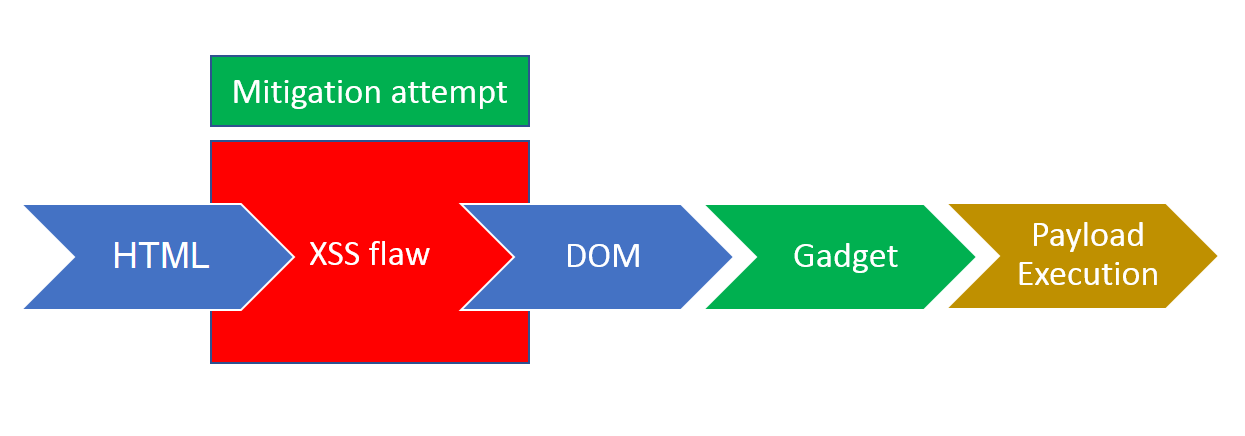
\includegraphics[width=\linewidth]{figures/attack_outline}
	\caption{Code-reuse attack outline}
	\label{fig:gadget_attack_outline}
\end{figure}



	\chapter{Gadgets in modern JS libraries}
In their paper \todo{Need to be completed} Sebastian Lekies et al. \cite{paper} the authors conducted an empirical study on 15 modern JavaScript libraries/frameworks. They looked manually at the code base of those libraries in order to find gadgets. So for each library in the list, they tried to build an exploit to bypass each of the mitigation tested. Interestingly, all the considered libraries\todo{Ref to code snippets may be leaked} (except for React) contain gadgets which can be abused to bypass different classes of mitigations. 

In order to describe this, It's best to start by looking at gadgets by the mitigations they target. 

\section{Bypassing WAFs \& XSS filters}
They detect XSS attepns by looking at request parameters, sometimes they use regular expressions and sometime they use more elaborate logic. If gadgets are really prevalent, they will be very successful in bypassing such mitigation, solely becuase of the way the gadgets work.  

\paragraph{Knockout.JS}
This is a Knockout JavaScript Library\todo{Add footnote}. This library has small templating language inside of it. The HTML snippet in listing \ref{lst:filters_knockout} tells Knockout to inject 'Hello World' as a string into the content of this \verb|<div>| element using some custom language for Knockout in specific. What this snippet in Knockout triggers is several gadgets. First Gadget, is very simple one, get the content of the \verb|data-bind| attribute and then assign it to some variable in the application. Later on, Knockout creates a JavaScript function and in the body of that function there is the 'Hello World' expression. Literally, there is a new function created by Knockout that will contain something originally present in the HTML that we assume injected. Finally, the Knockout will execute the newly created function will be the last gadget in the chain\todo{Gadget Chain idea}. To summaries, there is a gadget in Knockout that upgrade the value of \verb|data-bind| attribute into an \verb|eval()| call (the function constructor is essentially equivalent to \verb|eval()|).\\


\lstinputlisting[language=HTML,label={lst:filters_knockout},caption= tbd]{listings/knockout.html} 


\lstinputlisting[language=HTML,label={lst:filters_knockout_gadget},caption= Knockout gadgets chain that creates and executes a JS function]{listings/knockout_gadgets.js}

In summary, in order to XSS a website that happens to use the Knockout.js library, and also on top of that uses an XSS filter like WAF, and instead of injecting \verb|<script>| into the request, it is enough if you just inject this fairly-innocent-looking-to-the mitigation HTML element: 
\verb|<div data-bind="value: alert(1)"></div>|

\paragraph{Tooltip functionality in Bootstrap}
Bootstrap is another JS library which contain gadgets that are also capable of circumventing this class of mitigations. In Bootstrap we can define tooltips, The bootstrap does everything with data attributes via the so-called data attributes API. So here we have a tooltip and by default this tooltip is rendered as text. But as bootstrap functionality works by data attributes, you can change the internal configuration with bootstrap. So, you can assign data-html equals true which bootstrap will turn it into configuration property and it will use jQuery which will create a script node which will bypass strict-dynamic. 


\lstinputlisting[language=HTML,label={lst:bootstrap_tooltip},caption= tbd]{listings/bootstrap_tooltip.html}

\section{Bypassing HTML sanitizers}

Sometimes, web applications actually need to display untrusted HTML content coming from the user. Let’s take as an example a web mail application. That is where HTML sanitizers coming into place. They take the untrusted content, try to filter out everything bad that contains JS and leave everything else intact. For example, script elements will be removed, inline event handlers will be removed but the \verb|<p>| tag remains intact. Some sanitizers, often whitelist the data attribute ( a new to HTML specification). Those two properties allow some found Gadgets in modern JS library to be very handy in bypassing HTML sanitizers for two reasons:

\begin{enumerate}
	\item This JS code that we want to execute can be present in those benign attributes like id or title or other as you will see soon (that should not be presented like this in the final text).
	\item The gadgets very often leverage the data attributes value. So, they actually pulled part of the payload from the data-attributes. 
\end{enumerate}

\paragraph{Ajaxify}
Decides a div with class “document-script” should actually be created as script and the body of the div is the content of this newly created and initiated script. Such patterns are common and that is why Gadgets are interesting in bypassing mechanism. 

\lstinputlisting[language=HTML,label={lst:ajaxify},caption= tbd]{listings/ajaxify.html}

\paragraph{Bootstrap}
The same example as before (listing \ref{lst:bootstrap_tooltip})(the same vector) the simple gadgets can bypass both mitigations unmodified\todo{important idea to highlight}. 

\section{Bypassing CSP}
Content security policy works on a completely different level. They try to distinguish between a trusted script and untrusted script. To do this, it works on mode. 
	 
\begin{enumerate}
	\item Whitelist of origins.
	\item Nonce-based mode If the attacked injected a script 
\end{enumerate}

Unfortunately, it turned out that Content Security Policy is hard to adopt on existing website. Hard to adoption on existing website (cite). The community came up with a list of cures which makes the adoption a little bit easier on the expense of the security. 
\subsection{Bypassing CSP unsafe-eval} What it does to the policy is a slight relaxation. Now, your trusted script is allowed to call \verb|eval()| function. That looks benign  (safe), since the script is trusted and comes from trusted origin, what is the wose that can happen.

A lot of gadgets can bypass the unsafe-eval version of content security policy. simply because lots of gadgets call \verb|eval()|. 

\paragraph{Underscore.js}

library is a templating library: we can simply inject underscore template, and what ever is passed within those \verb|<% %>| will be passed to \verb|eval()| function for execution\todo{footnote}. 

\lstinputlisting[language=HTML,label={lst:underscore},caption= Bypassing CSP unsafe-eval with Underscore Gadget]{listings/underscore.html}

\subsection{Bypassing CSP strict-dynamic}
The second keyword. It’s most used in nonce-based mode. The problem is that a lot of script you include are unaware of this fact. Facebook like button as a script, or some other widgets those script will not aware that you are using CSP in nonce based mode so they will not be able to fetch those nonce and add them to the newly created scripts that these libraries create. What script dynamics does is that it allows trusted script to create new script without nonce. So, if you add a Facebook script that Facebook script can create new Facebook scripts without propagating trust. And this is interesting again since we can use (see) this in script gadgets. For example: Bypassing script-dynamic in jQuery mobile.

\lstinputlisting[language=HTML,label={lst:jquery_mobile},caption= Bypassing CSP strict-dynamic with jQuery Mobile Gadget]{listings/jquery_mobile.html}

jQuery Mobile has popup functionality, so you can press a button and you have this overlay popup. 
(For performance reason they prerendered it when the page load. Concatenate what is in the id as part of the comment for the popup placeholder. jQuery Mobile relies on jQuery.html() to render HTML). jQuery.html function is a wrapper for innerHTML function with one exception, it in addition to innerHTML tries to look for script tags in the string and creates them dynamically. That was work around by jQuery is the thing that allows as to have it as a gadget. (\verb|$.html()|  that behavior allows the HTML)

\subsection{Gadgets in expression parsers}
Now let’s get back to the traditional CSP (like without any unsafe-eval or strict-dynamic). Those getgets are hard to find. We couldn’t use any gadgets that will upgrage a text ito script using eval() since that is detected by CSP. Fortunatily, We where able to bypass such CSPs using gadgets in expression parsers. And as a bounus, the very same vector works for all other mitigations. 

\paragraph{Expression parsers}
There are several JS frameworks that have templating components inside them, so they have certain custom language for expression that could be embedded into the HTML. Let’s see how such expression may look like by taking an example from Aurelia framework. Listing \ref{lst:parser_example} . it instructs the Aurelia framework to insert the property name of some object called customer into the table element when rendering the page. What is interesting is that the code in braces is not JavaScript. It’s an expression written according to the definition of the expression language Aurelia framework. Which get parssed by Aurlia and then evaluate it. It creates a chain of function that would eventually fetch the name property of some customer object and then insert using, for example, \verb|innerHTML| or similar. 

\lstinputlisting[language=HTML,label={lst:parser_example},caption= tbd]{listings/parser_example.html}

Listing \ref{lst:aurelia_image_exploit} shows exploit for gadget in AnuglarJS expression parser. We have a cookie stealer that is completely JS free. That is completely JS free. In that expression, you tell Aurelia to take the global object which is window then give the document then put the cookie. And there is not JS involved. It’s a domain specific language of Aurelia. 

\lstinputlisting[language=HTML,label={lst:aurelia_image_exploit},caption= tbd]{listings/aurelia_image_exploit.html}

We can also do some interesting things, let’s suppose that CSP in place is in nonce-based mode to validate whether script is legitimate or not. We here use an expression to insert the nonce for us. Here in the example Let’s suppose the attacker inject the following, however, at injection time we don’t know the nonce. So we add a nonce attribute and within this nonce attribute we specify an expression: it will go to document and say what is the current script (in this case it’s Ractive ascript) and we get the nonce from there and add it in the current place.   

\lstinputlisting[language=HTML,label={lst:ractive},caption= tbd]{listings/ractive.html}

	\chapter{Script Gadgets in real-world apps}
% bibliography
% we recommend using cryptobib for your bibliography
% c.f. https://cryptobib.di.ens.fr
% you also might want use biblatex or bibtex. Add the packages as you like.
%\clearpage
%\addcontentsline{toc}{chapter}{Literaturverzeichnis}
%\bibliographystyle{alpha}
%\bibliography{abbrev0, crypto}

\printbibliography

\end{document}
